\begin{coqdoccode}
\end{coqdoccode}
\section{A Formalization of the Z property}


\begin{coqdoccode}
\end{coqdoccode}
An Abstract Reduction System (ARS) is a pair $(A,R)$, where \coqdocvar{A} is a set and \coqdocvar{R} is a binary relation over \coqdocvar{A} whose type written \coqdocvar{Rel} \coqdocvar{A} is defined as follows: 
\begin{coqdoccode}
\coqdocemptyline
\coqdocnoindent
\coqdockw{Definition} \coqdocvar{Rel} (\coqdocvar{A}:\coqdockw{Type}) := \coqdocvar{A} \ensuremath{\rightarrow} \coqdocvar{A} \ensuremath{\rightarrow} \coqdockw{Prop}.\coqdoceol
\coqdocemptyline
\end{coqdoccode}
Let $(A,R)$ be an ARS and $a,b\in A$. Then we write $a\to_R b$ (or $R\ a\ b$ in the Coq syntax below) to denote that $(a,b)\in R$, and in this case, we say that $a$ $R$-reduces to $b$ in one step. The reflexive transitive closure of $\to_R$, written $\tto_R$, is defined by:


\begin{mathpar}
     \inferrule*[Right={($refl$)}]{~}{a \tto_R a}\and\and
     \inferrule*[Right={($rtrans$)}]{a \to_R b \and b \tto_R c}{a \tto_R c}
\end{mathpar}


 This definition corresponds to the following Coq code, where $\tto_R$ is written as (\coqdocvar{refltrans} \coqdocvar{R}): 
\begin{coqdoccode}
\coqdocemptyline
\coqdocnoindent
\coqdockw{Inductive} \coqdocvar{refltrans} \{\coqdocvar{A}:\coqdockw{Type}\} (\coqdocvar{R}: \coqdocvar{Rel} \coqdocvar{A}) : \coqdocvar{A} \ensuremath{\rightarrow} \coqdocvar{A} \ensuremath{\rightarrow} \coqdockw{Prop} :=\coqdoceol
\coqdocnoindent
\ensuremath{|} \coqdocvar{refl}: \coqdockw{\ensuremath{\forall}} \coqdocvar{a}, \coqdocvar{refltrans} \coqdocvar{R} \coqdocvar{a} \coqdocvar{a}\coqdoceol
\coqdocnoindent
\ensuremath{|} \coqdocvar{rtrans}: \coqdockw{\ensuremath{\forall}} \coqdocvar{a} \coqdocvar{b} \coqdocvar{c}, \coqdocvar{R} \coqdocvar{a} \coqdocvar{b} \ensuremath{\rightarrow} \coqdocvar{refltrans} \coqdocvar{R} \coqdocvar{b} \coqdocvar{c} \ensuremath{\rightarrow} \coqdocvar{refltrans} \coqdocvar{R} \coqdocvar{a} \coqdocvar{c}.\coqdoceol
\end{coqdoccode}
The reflexive transitive closure of a relation is used to define
    the notion of confluence: no matter how the reduction is done, the
    result will always be the same. In other words, every divergence
    is joinable as stated by the following diagram:


    $\centerline{\xymatrix{ & a \ar@{->>}[dl] \ar@{->>}[dr] & \\ b
    \ar@{.>>}[dr] & & c \ar@{.>>}[dl] \\ & d & }}$


Formally, this means that if an expression $a$ can be reduced in two
different ways to $b$ and $c$, then there exists an expression $d$
such that both $b$ and $c$ reduce to $d$. The existential
quantification is expressed by the dotted lines in the diagram. This
notion is defined in the Coq system as follows: 
\begin{coqdoccode}
\coqdocemptyline
\coqdocnoindent
\coqdockw{Definition} \coqdocvar{Confl} \{\coqdocvar{A}:\coqdockw{Type}\} (\coqdocvar{R}: \coqdocvar{Rel} \coqdocvar{A}) := \coqdockw{\ensuremath{\forall}} \coqdocvar{a} \coqdocvar{b} \coqdocvar{c}, (\coqdocvar{refltrans} \coqdocvar{R}) \coqdocvar{a} \coqdocvar{b} \ensuremath{\rightarrow} (\coqdocvar{refltrans} \coqdocvar{R}) \coqdocvar{a} \coqdocvar{c} \ensuremath{\rightarrow} (\coqdoctac{\ensuremath{\exists}} \coqdocvar{d}, (\coqdocvar{refltrans} \coqdocvar{R}) \coqdocvar{b} \coqdocvar{d} \ensuremath{\land} (\coqdocvar{refltrans} \coqdocvar{R}) \coqdocvar{c} \coqdocvar{d}).\coqdoceol
\coqdocemptyline
\end{coqdoccode}
In \cite{dehornoy2008z}, V. van Oostrom gives a sufficient condition
for an ARS to be confluent. This condition is based on the $\textit{Z
  Property}$ that is defined as follows:


\begin{definition} Let $(A,\to_R)$ be an ARS. A mapping $f:A \to A$ satisfies the Z property for $\to_R$, if $a \to_R b$ implies
$b \tto_R f a  \tto_R f b$, for any $a, b \in A$. 
\end{definition}


The name of the property comes from the following diagrammatic
representation of this definition:


$\xymatrix{ a \ar[r]_R & b \ar@{.>>}[dl]^R\\ f a \ar@{.>>}[r]_R & f
    b \\ }$


If a function \coqdocvar{f} satisfies the Z property for $\to_R$ then
we say that \coqdocvar{f} is Z for $\to_R$, and the corresponding Coq
definition is given by the following predicate: 
\begin{coqdoccode}
\coqdocemptyline
\coqdocnoindent
\coqdockw{Definition} \coqdocvar{f\_is\_Z} \{\coqdocvar{A}:\coqdockw{Type}\} (\coqdocvar{R}: \coqdocvar{Rel} \coqdocvar{A}) (\coqdocvar{f}: \coqdocvar{A} \ensuremath{\rightarrow} \coqdocvar{A}) := \coqdockw{\ensuremath{\forall}} \coqdocvar{a} \coqdocvar{b}, \coqdocvar{R} \coqdocvar{a} \coqdocvar{b} \ensuremath{\rightarrow} ((\coqdocvar{refltrans} \coqdocvar{R})  \coqdocvar{b} (\coqdocvar{f} \coqdocvar{a}) \ensuremath{\land} (\coqdocvar{refltrans} \coqdocvar{R}) (\coqdocvar{f} \coqdocvar{a}) (\coqdocvar{f} \coqdocvar{b})).\coqdoceol
\coqdocemptyline
\end{coqdoccode}
Alternatively, an ARS $(A,\to_R)$ satisfies the Z property if there
exists a mapping $f:A \to A$ such that $f$ is Z for $\to_R$: 
\begin{coqdoccode}
\coqdocemptyline
\coqdocnoindent
\coqdockw{Definition} \coqdocvar{Z\_prop} \{\coqdocvar{A}:\coqdockw{Type}\} (\coqdocvar{R}: \coqdocvar{Rel} \coqdocvar{A}) := \coqdoctac{\ensuremath{\exists}} \coqdocvar{f}:\coqdocvar{A} \ensuremath{\rightarrow} \coqdocvar{A}, \coqdocvar{f\_is\_Z} \coqdocvar{R} \coqdocvar{f}.\coqdoceol
\coqdocemptyline
\end{coqdoccode}
The first contribution of this work is a constructive proof of the fact that the Z property implies confluence. Our proof uses nested induction, and hence it differs from the one in \cite{kesnerTheoryExplicitSubstitutions2009} (that follows \cite{dehornoy2008z}) and the one in \cite{felgenhauerProperty2016} in the sense that it does not rely on the analyses of whether a term is in normal form or not, avoiding the necessity of the law of the excluded middle. As a result, we have an elegant inductive proof of the fact that if an ARS satisfies the Z property then it is confluent. 
\begin{coqdoccode}
\coqdocemptyline
\coqdocnoindent
\coqdockw{Theorem} \coqdocvar{Z\_prop\_implies\_Confl} \{\coqdocvar{A}:\coqdockw{Type}\}: \coqdockw{\ensuremath{\forall}} \coqdocvar{R}: \coqdocvar{Rel} \coqdocvar{A}, \coqdocvar{Z\_prop} \coqdocvar{R} \ensuremath{\rightarrow} \coqdocvar{Confl} \coqdocvar{R}.\coqdoceol
\coqdocnoindent
\coqdockw{Proof}.\coqdoceol
\coqdocindent{1.00em}
\coqdoctac{intros} \coqdocvar{R} \coqdocvar{HZ\_prop}. \end{coqdoccode}
\comm{Let $R$ be a relation over $A$ that satisfies
    the Z property, which will be denoted by $HZ\_prop$ for future
    reference.} 
\begin{coqdoccode}
\coqdocemptyline
\coqdocindent{1.00em}
\coqdoctac{unfold} \coqdocvar{Z\_prop}, \coqdocvar{Confl} \coqdoctac{in} *. \end{coqdoccode}
\comm{Unfolding both definitions of
  $Z\_prop$ and $Confl$, we get the following proof context:

     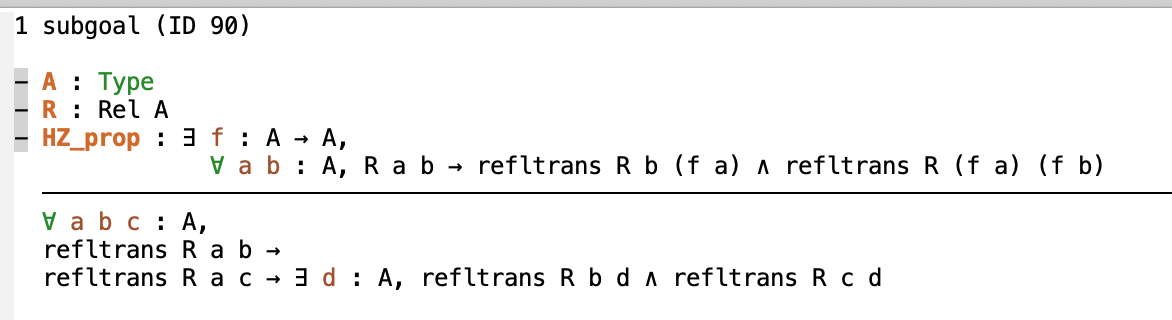
\includegraphics[scale=0.5]{figs/fig3.png} } 
\begin{coqdoccode}
\coqdocemptyline
\coqdocindent{1.00em}
\coqdoctac{intros} \coqdocvar{a} \coqdocvar{b} \coqdocvar{c} \coqdocvar{Hrefl1} \coqdocvar{Hrefl2}. \end{coqdoccode}
\comm{Let $a, b$ and $c$ be elements of
     the set $A$, $Hrefl1$ the hypothesis that $a \tto_R b$, and
     $Hrefl2$ the hypothesis that $a\tto_R c$. We need to prove that
     there exists $d$ such that $b\tto_R d$ and $c\tto_R d$.} 
\begin{coqdoccode}
\coqdocemptyline
\coqdocindent{1.00em}
\coqdoctac{destruct} \coqdocvar{HZ\_prop} \coqdockw{as} [\coqdocvar{g} \coqdocvar{HZ\_prop}]. \end{coqdoccode}
\comm{We know from the hypothesis
     $HZ\_prop$ that there exists a mapping $f$ that is Z. Let's call
     $g$ this mapping, and we get following proof context:

      \symbol{92}includegraphics\coqdocvar{scale}=0.6\{figs/fig4.png\}

      The proof proceeds by nested induction, firstly on the length of
      the reduction from $a$ to $b$, and then on the length of the
      reduction from $a$ to $c$.} 
\begin{coqdoccode}
\coqdocemptyline
\coqdocindent{1.00em}
\coqdoctac{generalize} \coqdoctac{dependent} \coqdocvar{c}. \end{coqdoccode}
\comm{Before the first induction,
      i.e. induction on $Hrefl1$, the element $c$ needs to be
      generalized so that it can be afterwards instantiated with any
      reduct of $a$.} 
\begin{coqdoccode}
\coqdocemptyline
\coqdocindent{1.00em}
\coqdoctac{induction} \coqdocvar{Hrefl1}. \end{coqdoccode}
\comm{The induction on $Hrefl1$ corresponds to
       induction on the reflexive transitive closure of the relation
       $R$, and since $refltrans$ has two rules, the goal splits in
       two subgoals, one for each possible way of constructing $a
       \tto_R b$.} 
\begin{coqdoccode}
\coqdocemptyline
\coqdocindent{1.00em}
- \coqdoctac{intros} \coqdocvar{c} \coqdocvar{Hrefl2}. \end{coqdoccode}
\comm{In the first case, we have that $b = a$ since
    we are in the reflexive case. This means that we have to prove
    that there exists $d$, such that $a \tto_R d$ and $c \tto_R d$.} 
\begin{coqdoccode}
\coqdocemptyline
\coqdocindent{2.00em}
\coqdoctac{\ensuremath{\exists}} \coqdocvar{c}; \coqdoctac{split}. \end{coqdoccode}
\comm{Taking $d$ as $c$, the proof is simplified to $a
    \tto_R c$ and $c \tto_R c$.} 
\begin{coqdoccode}
\coqdocemptyline
\coqdocindent{2.00em}
+ \coqdoctac{assumption}. \end{coqdoccode}
\comm{The first component is exactly the hypothesis
        $Hrefl2$ and } 
\begin{coqdoccode}
\coqdocemptyline
\coqdocindent{2.00em}
+ \coqdoctac{apply} \coqdocvar{refl}. \end{coqdoccode}
\comm{$c \tto_R c$ corresponds to an application of
        the $refl$ axiom.} 

 The interesting part of the proof is then given by the
        inductive case, i.e. when $a\tto_R b$ is generated by the rule
        (\coqdocvar{rtrans}). In this case, the reduction from \coqdocvar{a} to \coqdocvar{b} is
        done in at least one step, therefore there must exists an
        element $a'$ such that the following diagram holds.


         \[\xymatrix{ & & a \ar@{->}[dl] \ar@{->>}[dr] & \\ & a'
        \ar@{->>}[dl] & & c \ar@{.>>}[ddll] \\ b \ar@{.>>}[dr] & & &
        \\ & d & & }\]  


        

        The induction hypothesis states that every divergence from
        $a'$ that reduces to $b$ from one side converges: \coqdocvar{IHHrefl1}
        : $\forall c_0 : A, a'\tto_R c_0 \to (\exists d : A, b\tto_R d
        \land c_0\tto_R d$). Now, we'd like apply induction on the
        hypothesis \coqdocvar{Hrefl2} (a\symbol{92}tto\_R c), but the current proof context has the
        hypothesis \coqdocvar{H}: $a\to_R a'$ (\coqdocvar{a} reduces to \coqdocvar{a'} in one step),
        and hence it is the sole hypothesis depending on \coqdocvar{a} in the
        current proof context. If we were to apply induction on \coqdocvar{Hrefl2} now, 
        the generated induction hypothesis \coqdocvar{IHrefl2} would assume that there is 
        a term $a''$ such that $a \to_R a'' \tto_R c$ and would require that 
        $a'' \to_R a'$, which is generally false. In order to circumvent 
        this problem, we need to discard the hypothesis \coqdocvar{H} from our proof 
        context, and replace it by another relevant information derived from 
        the Z property as shown in what follows. 
\begin{coqdoccode}
\coqdocemptyline
\coqdocindent{1.00em}
- \coqdoctac{intros} \coqdocvar{c0} \coqdocvar{Hrefl2}. \end{coqdoccode}
\comm{Let $c_0$ be a reduct of $a$, and $Hrefl2$
    be the hypothesis $a \tto_R c_0$. So the reduction $a\tto_R c$ in
    the above diagram is now $a\tto_R c_0$ due to a renaming of
    variables automatically done by the Coq system. In addition, the
    reduction $a \to_R a' \tto_R b$ is now $a\to_R b \tto_R c$, as
    shown below:

    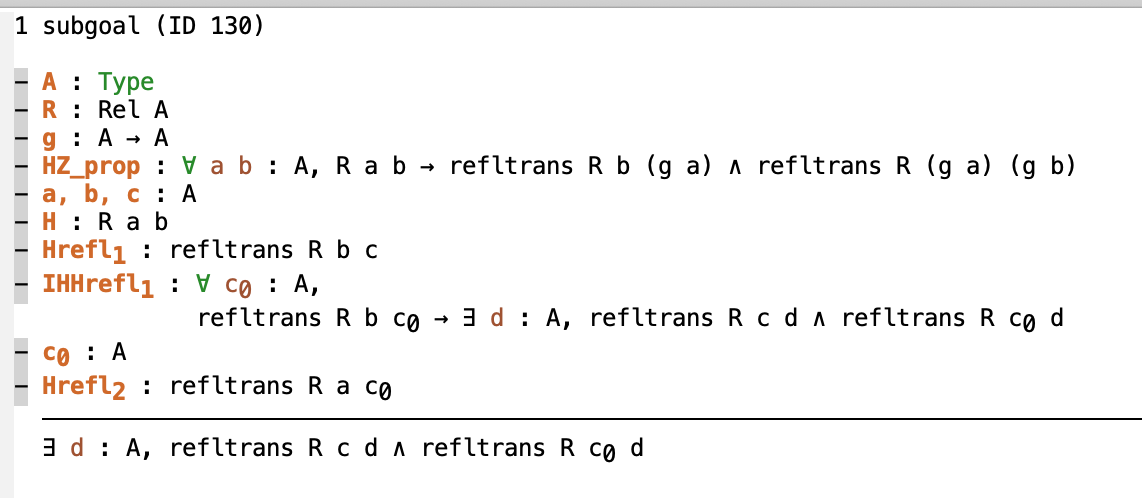
\includegraphics[scale=0.5]{figs/fig5-1.png}

    Before applying induction to $Hrefl2$: $a \tto_R c_0$, we will derive 
    $b\tto_R (g\ a)$ and $a\tto_R (g\ a)$ from the proof context so we can
    discard the hypothesis $H$: $a\to_R$.} 
\begin{coqdoccode}
\coqdocemptyline
\coqdocindent{2.00em}
\coqdoctac{assert} (\coqdocvar{Hbga}: \coqdocvar{refltrans} \coqdocvar{R} \coqdocvar{b} (\coqdocvar{g} \coqdocvar{a})).\coqdoceol
\coqdocindent{2.00em}
\{ \coqdoctac{apply} \coqdocvar{HZ\_prop}; \coqdoctac{assumption}. \} \end{coqdoccode}
\comm{We call $Hbga$ the reduction
    $b\tto_R (g\ a)$ that is directly obtained from the Z property.} 
\begin{coqdoccode}
\coqdocnoindent
\coqdoceol
\coqdocindent{2.00em}
\coqdoctac{assert} (\coqdocvar{Haga}: \coqdocvar{refltrans} \coqdocvar{R} \coqdocvar{a} (\coqdocvar{g} \coqdocvar{a})).\coqdoceol
\coqdocindent{2.00em}
\{ \coqdoctac{apply} \coqdocvar{rtrans} \coqdockw{with} \coqdocvar{b}; \coqdoctac{assumption}. \} \end{coqdoccode}
\comm{Call $Haga$ the
        reduction $a\tto_R (g\ a)$, and prove it using the
        transitivity of $\tto_R$, since $a \to_R b$ and $b \tto_R (g\
        a)$. Diagrammatically, we change from the situation on the
        top to the bottomone on the right:

        \xymatrix{ & & a \ar@{->>}[ddrr]_R \ar@{->}[dl]^R & & \\ & b
        \ar@{->>}[dl]^R & & & \\ c \ar@{.>>}[ddrr]_R & & & & c_0
        \ar@{.>>}[ddll]^R \\ & & & & \\ & & d & & } 

        \xymatrix{ & & a \ar@{->>}[ddrr]_R \ar@{->>}[dd]_R & & \\ & b
        \ar@{->>}[dl]^R \ar@{->>}[dr]_R & & & \\ c \ar@{.>>}[ddrr]_R &
        & (g \; a) & & c_0 \ar@{.>>}[ddll]^R \\ & & & & \\ & & d & &} } 
\begin{coqdoccode}
\coqdocnoindent
\coqdoceol
\coqdocindent{2.00em}
\coqdoctac{clear} \coqdocvar{H}. \coqdoctac{generalize} \coqdoctac{dependent} \coqdocvar{b}. \end{coqdoccode}
\comm{At this point we can remove
      the hypothesis $H$ from the context, and generalize $b$. Doing so, 
      we generalize $IHHrefl1$, which, in conjunction with the hypotheses 
      that depend on a (namely, $Hrefl2$, $Hbga$, and $Haga$), will form 
      the four necessary conditions for use of the second inductive 
      hypothesis, $IHHrefl2$.} 
\begin{coqdoccode}
\coqdocemptyline
\coqdocindent{2.00em}
\coqdoctac{induction} \coqdocvar{Hrefl2}. \end{coqdoccode}
\comm{Now we are ready to start the induction on
    the reduction $a\tto_R c_0$, and we have two subgoals.} 
\begin{coqdoccode}
\coqdocemptyline
\coqdocindent{2.00em}
+ \coqdoctac{intros} \coqdocvar{b} \coqdocvar{Hrefl1} \coqdocvar{IHHrefl1} \coqdocvar{Hbga}. \end{coqdoccode}
\comm{The first subgoal corresponds
        to the reflexive case that is closed by the induction
        hypothesis $IHHrefl1$:

        \[\xymatrix{ & & a \ar@{->>}[dd]^{H2} & & \\ & b
        \ar@{->>}[dl]_{Hrefl1} \ar@{->>}[dr]^{H1} & & & \\ c
        \ar@{.>>}[dr] & IHHrefl1 & (g \; a) \ar@{.>>}[dl] & & \\ & d &
        &&}\] } 
\begin{coqdoccode}
\coqdocemptyline
\coqdocindent{3.00em}
\coqdoctac{assert} (\coqdocvar{IHHrefl1\_ga} := \coqdocvar{IHHrefl1} (\coqdocvar{g} \coqdocvar{a}));\coqdoceol
\coqdocindent{4.00em}
\coqdoceol
\coqdocindent{4.00em}
\coqdoctac{apply} \coqdocvar{IHHrefl1\_ga} \coqdoctac{in} \coqdocvar{Hbga}. \end{coqdoccode}
\comm{In order to apply $IHHrefl1$, we instantiate $c_0$ with $(g\
      a)$.} 
\begin{coqdoccode}
\coqdocemptyline
\coqdocindent{3.00em}
\coqdoctac{destruct} \coqdocvar{Hbga}. \end{coqdoccode}
\comm{Therefore, there exists an element, say $x$,
      such that both $c\tto_R x$ and $(g\ a) \tto_R x$.} 
\begin{coqdoccode}
\coqdocemptyline
\coqdocindent{3.00em}
\coqdoctac{\ensuremath{\exists}} \coqdocvar{x}; \coqdoctac{split}. \end{coqdoccode}
\comm{We then take $x$ to show that $c\tto_R x$ and $a
      \tto_R x$.} 
\begin{coqdoccode}
\coqdocemptyline
\coqdocindent{3.00em}
\ensuremath{\times} \coqdoctac{apply} \coqdocvar{H}. \end{coqdoccode}
\comm{Note that $c\tto_R x$ is already an hypothesis,
        and we are done.} 
\begin{coqdoccode}
\coqdocemptyline
\coqdocindent{3.00em}
\ensuremath{\times} \coqdoctac{apply} \coqdocvar{refltrans\_composition} \coqdockw{with} (\coqdocvar{g} \coqdocvar{a});\coqdoceol
\coqdocnoindent
\coqdoceol
\coqdocindent{4.00em}
[\coqdoctac{assumption} \ensuremath{|} \coqdoctac{apply} \coqdocvar{H}]. \end{coqdoccode}
      \comm{The proof of $a \tto_R x$ is done by the transitivity of
      $\tto_R$ taking $(g\ a)$ as the intermediate step.} 
\begin{coqdoccode}
\coqdocemptyline
\coqdocindent{2.00em}
+ \coqdoctac{intros} \coqdocvar{b0} \coqdocvar{Hrefl1} \coqdocvar{IHHrefl1} \coqdocvar{Hb0ga}. \end{coqdoccode}
\comm{The second subgoal corresponds
        to the case in which $a\tto_R c_0$ is generated by the rule
        $(rtrans)$. Therefore, there exists a term $b$ such that
        $a\to_R b$ and $b \tto_R c_0$. The corresponding proof context
        after introducing the universally quantified variable $b0$,
        the hypothesis $Hrefl1$ and the induction hypothesis
        $IHHrefl1$ generated by the first outer induction and the fact
        that $b0 \tto_R (g\ a)$ is given by:

        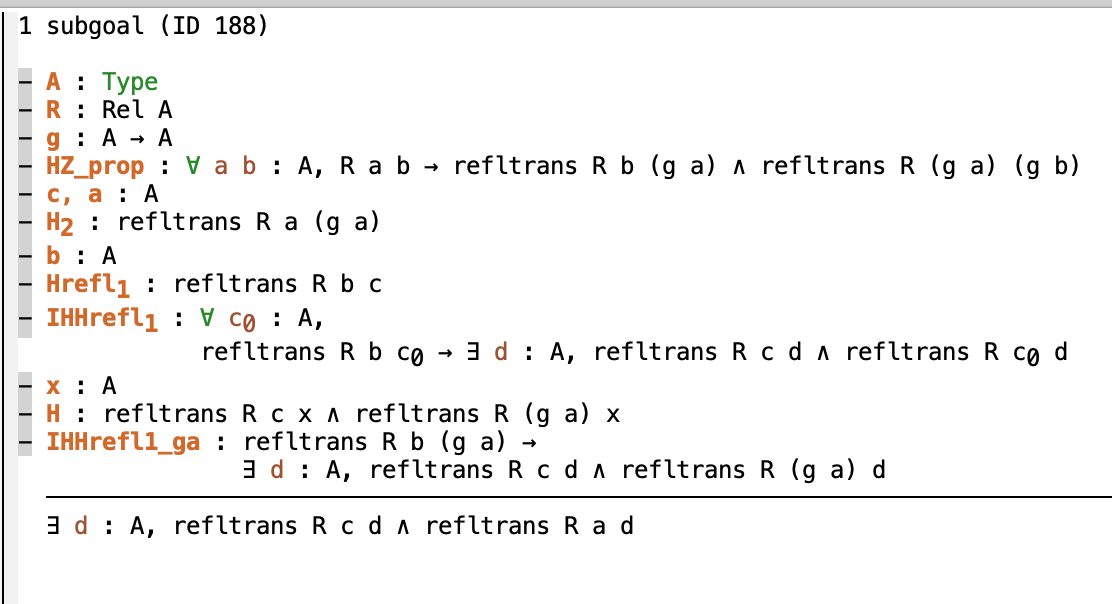
\includegraphics[scale=0.48]{figs/fig7.png} } 
\begin{coqdoccode}
\coqdocemptyline
\coqdocindent{3.00em}
\coqdoctac{apply} \coqdocvar{IHHrefl2} \coqdockw{with} \coqdocvar{b0}. \end{coqdoccode}
\comm{The second goal, i.e. the inductive case is 
      the consequent on $IHHrefl2$, so we can apply $IHHrefl2$ to prove it. Doing so, 
      we must prove the antecedent of $IHHrefl2$, which consists of four separate 
      hypotheses that we must prove. Those hypotheses are as follows:} 
\begin{coqdoccode}
\coqdocemptyline
\coqdocindent{3.00em}
\ensuremath{\times} \coqdoctac{apply} \coqdocvar{refltrans\_composition} \coqdockw{with} (\coqdocvar{g} \coqdocvar{a});\coqdoceol
\coqdocindent{5.00em}
\coqdoceol
\coqdocindent{4.00em}
\coqdoctac{apply} \coqdocvar{HZ\_prop}; \coqdoctac{assumption}. \end{coqdoccode}
\comm{1. $b \tto_R (g\ b)$: This is proved by the transitivity of the
      reflexive transitive closure of $R$ using the
      hypothesis (H: $a\to_R b$) and $HZ\_prop$: $\forall a\
      b: a \to_R b \to (b \tto_R (g\ a) \land (g\ a) \tto_R (g\ b))$.} 
\begin{coqdoccode}
\coqdocemptyline
\coqdocindent{3.00em}
\ensuremath{\times} \coqdoctac{assumption}. \end{coqdoccode}
\comm{2. $b0 \tto_R c$: This is exactly the
          hypothesis $Hrefl1$.} 
\begin{coqdoccode}
\coqdocemptyline
\coqdocindent{3.00em}
\ensuremath{\times} \coqdoctac{assumption}. \end{coqdoccode}
\comm{3. $\forall c0: b0 \tto_R c0 \to (\exists d:
            c \tto_R d \land c0 \tto_R d)$: This is exactly the
            induction hypothesis $IHHrefl1$.} 
\begin{coqdoccode}
\coqdocemptyline
\coqdocindent{3.00em}
\ensuremath{\times} \coqdoctac{apply} \coqdocvar{refltrans\_composition} \coqdockw{with} (\coqdocvar{g} \coqdocvar{a});\coqdoceol
\coqdocindent{4.00em}
[ \coqdoctac{assumption} \ensuremath{|} \coqdoctac{apply} \coqdocvar{HZ\_prop}; \coqdoctac{assumption}]. \end{coqdoccode}
\comm{4. $b0 \tto_R (g\ b)$: This is proved by the transitivity of
      the reflexive transitive closure of $R$ using the
      hypothesis $H'$: $b0 \tto_R (g\ a)$ and the fact that
      $(g\ a) \tto_R (g\ b)$ that is obtained from the fact that
      $R$ satisfies the Z property (hypothesis
      $HZ\_prop$).} 
\begin{coqdoccode}
\coqdocemptyline
\coqdocnoindent
\coqdockw{Qed}.\coqdoceol
\coqdocemptyline
\coqdocnoindent
\coqdockw{Definition} \coqdocvar{SemiConfl} \{\coqdocvar{A}:\coqdockw{Type}\} (\coqdocvar{R}: \coqdocvar{Rel} \coqdocvar{A}) := \coqdockw{\ensuremath{\forall}} \coqdocvar{a} \coqdocvar{b} \coqdocvar{c}, \coqdocvar{R} \coqdocvar{a} \coqdocvar{b} \ensuremath{\rightarrow} (\coqdocvar{refltrans} \coqdocvar{R}) \coqdocvar{a} \coqdocvar{c} \ensuremath{\rightarrow} (\coqdoctac{\ensuremath{\exists}} \coqdocvar{d}, (\coqdocvar{refltrans} \coqdocvar{R}) \coqdocvar{b} \coqdocvar{d} \ensuremath{\land} (\coqdocvar{refltrans} \coqdocvar{R}) \coqdocvar{c} \coqdocvar{d}).\coqdoceol
\coqdocemptyline
\coqdocnoindent
\coqdockw{Theorem} \coqdocvar{Z\_prop\_implies\_SemiConfl} \{\coqdocvar{A}:\coqdockw{Type}\}: \coqdockw{\ensuremath{\forall}} \coqdocvar{R}: \coqdocvar{Rel} \coqdocvar{A}, \coqdocvar{Z\_prop} \coqdocvar{R} \ensuremath{\rightarrow} \coqdocvar{SemiConfl} \coqdocvar{R}.\coqdoceol
\coqdocemptyline
\coqdocnoindent
\coqdockw{Theorem} \coqdocvar{Semi\_equiv\_Confl} \{\coqdocvar{A}: \coqdockw{Type}\}: \coqdockw{\ensuremath{\forall}} \coqdocvar{R}: \coqdocvar{Rel} \coqdocvar{A}, \coqdocvar{Confl} \coqdocvar{R} \ensuremath{\leftrightarrow} \coqdocvar{SemiConfl} \coqdocvar{R}.\coqdoceol
\coqdocemptyline
\coqdocnoindent
\coqdockw{Corollary} \coqdocvar{Zprop\_implies\_Confl\_via\_SemiConfl} \{\coqdocvar{A}:\coqdockw{Type}\}: \coqdockw{\ensuremath{\forall}} \coqdocvar{R}: \coqdocvar{Rel} \coqdocvar{A}, \coqdocvar{Z\_prop} \coqdocvar{R} \ensuremath{\rightarrow} \coqdocvar{Confl} \coqdocvar{R}.\coqdoceol
\coqdocemptyline
\end{coqdoccode}
\section{An extension of the Z property: Compositional Z}


\begin{coqdoccode}
\coqdocemptyline
\coqdocnoindent
\coqdockw{Definition} \coqdocvar{f\_is\_weak\_Z} \{\coqdocvar{A}\} (\coqdocvar{R} \coqdocvar{R'}: \coqdocvar{Rel} \coqdocvar{A}) (\coqdocvar{f}: \coqdocvar{A} \ensuremath{\rightarrow} \coqdocvar{A}) := \coqdockw{\ensuremath{\forall}} \coqdocvar{a} \coqdocvar{b}, \coqdocvar{R} \coqdocvar{a} \coqdocvar{b} \ensuremath{\rightarrow} ((\coqdocvar{refltrans} \coqdocvar{R'}) \coqdocvar{b} (\coqdocvar{f} \coqdocvar{a}) \ensuremath{\land} (\coqdocvar{refltrans} \coqdocvar{R'}) (\coqdocvar{f} \coqdocvar{a}) (\coqdocvar{f} \coqdocvar{b})).\coqdoceol
\coqdocemptyline
\coqdocnoindent
\coqdockw{Definition} \coqdocvar{comp} \{\coqdocvar{A}\} (\coqdocvar{f1} \coqdocvar{f2}: \coqdocvar{A} \ensuremath{\rightarrow} \coqdocvar{A}) := \coqdockw{fun} \coqdocvar{x}:\coqdocvar{A} \ensuremath{\Rightarrow} \coqdocvar{f1} (\coqdocvar{f2} \coqdocvar{x}).\coqdoceol
\coqdocnoindent
\coqdockw{Notation} "f1 \# f2" := (\coqdocvar{comp} \coqdocvar{f1} \coqdocvar{f2}) (\coqdoctac{at} \coqdockw{level} 40).\coqdoceol
\coqdocemptyline
\coqdocnoindent
\coqdockw{Inductive} \coqdocvar{union} \{\coqdocvar{A}\} (\coqdocvar{red1} \coqdocvar{red2}: \coqdocvar{Rel} \coqdocvar{A}) : \coqdocvar{Rel} \coqdocvar{A} :=\coqdoceol
\coqdocnoindent
\ensuremath{|} \coqdocvar{union\_left}: \coqdockw{\ensuremath{\forall}} \coqdocvar{a} \coqdocvar{b}, \coqdocvar{red1} \coqdocvar{a} \coqdocvar{b} \ensuremath{\rightarrow} \coqdocvar{union} \coqdocvar{red1} \coqdocvar{red2} \coqdocvar{a} \coqdocvar{b}\coqdoceol
\coqdocnoindent
\ensuremath{|} \coqdocvar{union\_right}: \coqdockw{\ensuremath{\forall}} \coqdocvar{a} \coqdocvar{b}, \coqdocvar{red2} \coqdocvar{a} \coqdocvar{b} \ensuremath{\rightarrow} \coqdocvar{union} \coqdocvar{red1} \coqdocvar{red2} \coqdocvar{a} \coqdocvar{b}.\coqdoceol
\coqdocnoindent
\coqdockw{Notation} "R1 !\_! R2" := (\coqdocvar{union} \coqdocvar{R1} \coqdocvar{R2}) (\coqdoctac{at} \coqdockw{level} 40).\coqdoceol
\coqdocemptyline
\coqdocnoindent
\coqdockw{Lemma} \coqdocvar{union\_or} \{\coqdocvar{A}\}: \coqdockw{\ensuremath{\forall}} (\coqdocvar{r1} \coqdocvar{r2}: \coqdocvar{Rel} \coqdocvar{A}) (\coqdocvar{a} \coqdocvar{b}: \coqdocvar{A}), (\coqdocvar{r1} !\coqdocvar{\_}! \coqdocvar{r2}) \coqdocvar{a} \coqdocvar{b} \ensuremath{\leftrightarrow} (\coqdocvar{r1} \coqdocvar{a} \coqdocvar{b}) \ensuremath{\lor} (\coqdocvar{r2} \coqdocvar{a} \coqdocvar{b}).\coqdoceol
\coqdocnoindent
\coqdockw{Require} \coqdockw{Import} \coqdocvar{Setoid}.\coqdoceol
\coqdocnoindent
\coqdockw{Require} \coqdockw{Import} \coqdocvar{ZArith}.\coqdoceol
\coqdocemptyline
\coqdocnoindent
\coqdockw{Lemma} \coqdocvar{equiv\_refltrans} \{\coqdocvar{A}\}: \coqdockw{\ensuremath{\forall}} (\coqdocvar{R} \coqdocvar{R1} \coqdocvar{R2}: \coqdocvar{Rel} \coqdocvar{A}), (\coqdockw{\ensuremath{\forall}} \coqdocvar{x} \coqdocvar{y}, \coqdocvar{R} \coqdocvar{x} \coqdocvar{y} \ensuremath{\leftrightarrow} (\coqdocvar{R1} !\coqdocvar{\_}! \coqdocvar{R2}) \coqdocvar{x} \coqdocvar{y}) \ensuremath{\rightarrow} \coqdockw{\ensuremath{\forall}} \coqdocvar{x} \coqdocvar{y}, \coqdocvar{refltrans} (\coqdocvar{R1} !\coqdocvar{\_}! \coqdocvar{R2}) \coqdocvar{x} \coqdocvar{y} \ensuremath{\rightarrow} \coqdocvar{refltrans} \coqdocvar{R} \coqdocvar{x} \coqdocvar{y}.\coqdoceol
\coqdocemptyline
\coqdocnoindent
\coqdockw{Definition} \coqdocvar{Z\_comp} \{\coqdocvar{A}:\coqdockw{Type}\} (\coqdocvar{R} :\coqdocvar{Rel} \coqdocvar{A}) := \coqdoctac{\ensuremath{\exists}} (\coqdocvar{R1} \coqdocvar{R2}: \coqdocvar{Rel} \coqdocvar{A}) (\coqdocvar{f1} \coqdocvar{f2}: \coqdocvar{A} \ensuremath{\rightarrow} \coqdocvar{A}), (\coqdockw{\ensuremath{\forall}} \coqdocvar{x} \coqdocvar{y}, \coqdocvar{R} \coqdocvar{x} \coqdocvar{y} \ensuremath{\leftrightarrow} (\coqdocvar{R1} !\coqdocvar{\_}! \coqdocvar{R2}) \coqdocvar{x} \coqdocvar{y}) \ensuremath{\land} \coqdocvar{f\_is\_Z} \coqdocvar{R1} \coqdocvar{f1} \ensuremath{\land} (\coqdockw{\ensuremath{\forall}} \coqdocvar{a} \coqdocvar{b}, \coqdocvar{R1} \coqdocvar{a} \coqdocvar{b} \ensuremath{\rightarrow} (\coqdocvar{refltrans} \coqdocvar{R}) ((\coqdocvar{f2} \# \coqdocvar{f1}) \coqdocvar{a}) ((\coqdocvar{f2} \# \coqdocvar{f1}) \coqdocvar{b})) \ensuremath{\land} (\coqdockw{\ensuremath{\forall}} \coqdocvar{a} \coqdocvar{b}, \coqdocvar{b} = \coqdocvar{f1} \coqdocvar{a} \ensuremath{\rightarrow} (\coqdocvar{refltrans} \coqdocvar{R}) \coqdocvar{b} (\coqdocvar{f2} \coqdocvar{b})) \ensuremath{\land} (\coqdocvar{f\_is\_weak\_Z} \coqdocvar{R2} \coqdocvar{R} (\coqdocvar{f2} \# \coqdocvar{f1})).\coqdoceol
\coqdocemptyline
\coqdocnoindent
\coqdockw{Lemma} \coqdocvar{refltrans\_union} \{\coqdocvar{A}:\coqdockw{Type}\}: \coqdockw{\ensuremath{\forall}} (\coqdocvar{R} \coqdocvar{R'} :\coqdocvar{Rel} \coqdocvar{A}) (\coqdocvar{a} \coqdocvar{b}: \coqdocvar{A}), \coqdocvar{refltrans} \coqdocvar{R} \coqdocvar{a} \coqdocvar{b} \ensuremath{\rightarrow} \coqdocvar{refltrans} (\coqdocvar{R} !\coqdocvar{\_}! \coqdocvar{R'}) \coqdocvar{a} \coqdocvar{b}.\coqdoceol
\coqdocemptyline
\coqdocnoindent
\coqdockw{Require} \coqdockw{Import} \coqdocvar{Setoid}.\coqdoceol
\coqdocnoindent
\coqdockw{Lemma} \coqdocvar{refltrans\_union\_equiv} \{\coqdocvar{A}\}: \coqdockw{\ensuremath{\forall}} (\coqdocvar{R} \coqdocvar{R1} \coqdocvar{R2} : \coqdocvar{Rel} \coqdocvar{A}), (\coqdockw{\ensuremath{\forall}} (\coqdocvar{x} \coqdocvar{y} : \coqdocvar{A}), (\coqdocvar{R} \coqdocvar{x} \coqdocvar{y} \ensuremath{\leftrightarrow} (\coqdocvar{R1} !\coqdocvar{\_}! \coqdocvar{R2}) \coqdocvar{x} \coqdocvar{y})) \ensuremath{\rightarrow} \coqdockw{\ensuremath{\forall}} (\coqdocvar{x} \coqdocvar{y}: \coqdocvar{A}), \coqdocvar{refltrans} (\coqdocvar{R1} !\coqdocvar{\_}! \coqdocvar{R2}) \coqdocvar{x} \coqdocvar{y} \ensuremath{\rightarrow} \coqdocvar{refltrans} \coqdocvar{R} \coqdocvar{x} \coqdocvar{y}.\coqdoceol
\coqdocemptyline
\coqdocnoindent
\coqdockw{Theorem} \coqdocvar{Z\_comp\_implies\_Z\_prop} \{\coqdocvar{A}:\coqdockw{Type}\}: \coqdockw{\ensuremath{\forall}} (\coqdocvar{R} :\coqdocvar{Rel} \coqdocvar{A}), \coqdocvar{Z\_comp} \coqdocvar{R} \ensuremath{\rightarrow} \coqdocvar{Z\_prop} \coqdocvar{R}.\coqdoceol
\coqdocemptyline
\end{coqdoccode}
Now we can use the proofs of the theorems \coqdocvar{Z\_comp\_implies\_Z\_prop}
and \coqdocvar{Z\_prop\_implies\_Confl} to conclude that compositional Z is a
sufficient condition for confluence. 
\begin{coqdoccode}
\coqdocemptyline
\coqdocnoindent
\coqdockw{Corollary} \coqdocvar{Z\_comp\_is\_Confl} \{\coqdocvar{A}\}: \coqdockw{\ensuremath{\forall}} (\coqdocvar{R}: \coqdocvar{Rel} \coqdocvar{A}), \coqdocvar{Z\_comp} \coqdocvar{R} \ensuremath{\rightarrow} \coqdocvar{Confl} \coqdocvar{R}.\coqdoceol
\coqdocemptyline
\coqdocnoindent
\coqdockw{Theorem} \coqdocvar{Z\_comp\_thm} \{\coqdocvar{A}:\coqdockw{Type}\}: \coqdockw{\ensuremath{\forall}} (\coqdocvar{R} :\coqdocvar{Rel} \coqdocvar{A}) (\coqdocvar{R1} \coqdocvar{R2}: \coqdocvar{Rel} \coqdocvar{A}) (\coqdocvar{f1} \coqdocvar{f2}: \coqdocvar{A} \ensuremath{\rightarrow} \coqdocvar{A}), (\coqdockw{\ensuremath{\forall}} \coqdocvar{x} \coqdocvar{y}, \coqdocvar{R} \coqdocvar{x} \coqdocvar{y} \ensuremath{\leftrightarrow} (\coqdocvar{R1} !\coqdocvar{\_}! \coqdocvar{R2}) \coqdocvar{x} \coqdocvar{y}) \ensuremath{\land} \coqdocvar{f\_is\_Z} \coqdocvar{R1} \coqdocvar{f1} \ensuremath{\land} (\coqdockw{\ensuremath{\forall}} \coqdocvar{a} \coqdocvar{b}, \coqdocvar{R1} \coqdocvar{a} \coqdocvar{b} \ensuremath{\rightarrow} (\coqdocvar{refltrans} \coqdocvar{R}) ((\coqdocvar{f2} \# \coqdocvar{f1}) \coqdocvar{a}) ((\coqdocvar{f2} \# \coqdocvar{f1}) \coqdocvar{b})) \ensuremath{\land} (\coqdockw{\ensuremath{\forall}} \coqdocvar{a} \coqdocvar{b}, \coqdocvar{b} = \coqdocvar{f1} \coqdocvar{a} \ensuremath{\rightarrow} (\coqdocvar{refltrans} \coqdocvar{R}) \coqdocvar{b} (\coqdocvar{f2} \coqdocvar{b})) \ensuremath{\land} (\coqdocvar{f\_is\_weak\_Z} \coqdocvar{R2} \coqdocvar{R} (\coqdocvar{f2} \# \coqdocvar{f1})) \ensuremath{\rightarrow} \coqdocvar{f\_is\_Z} \coqdocvar{R} (\coqdocvar{f2} \# \coqdocvar{f1}).\coqdoceol
\coqdocemptyline
\coqdocnoindent
\coqdockw{Corollary} \coqdocvar{Z\_comp\_eq\_corol} \{\coqdocvar{A}:\coqdockw{Type}\}: \coqdockw{\ensuremath{\forall}} (\coqdocvar{R} :\coqdocvar{Rel} \coqdocvar{A}) (\coqdocvar{R1} \coqdocvar{R2}: \coqdocvar{Rel} \coqdocvar{A}) (\coqdocvar{f1} \coqdocvar{f2}: \coqdocvar{A} \ensuremath{\rightarrow} \coqdocvar{A}), (\coqdockw{\ensuremath{\forall}} \coqdocvar{x} \coqdocvar{y}, \coqdocvar{R} \coqdocvar{x} \coqdocvar{y} \ensuremath{\leftrightarrow} (\coqdocvar{R1} !\coqdocvar{\_}! \coqdocvar{R2}) \coqdocvar{x} \coqdocvar{y}) \ensuremath{\land} (\coqdockw{\ensuremath{\forall}} \coqdocvar{a} \coqdocvar{b}, \coqdocvar{R1} \coqdocvar{a} \coqdocvar{b} \ensuremath{\rightarrow} (\coqdocvar{f1} \coqdocvar{a}) = (\coqdocvar{f1} \coqdocvar{b})) \ensuremath{\land} (\coqdockw{\ensuremath{\forall}} \coqdocvar{a}, (\coqdocvar{refltrans} \coqdocvar{R1}) \coqdocvar{a} (\coqdocvar{f1} \coqdocvar{a})) \ensuremath{\land} (\coqdockw{\ensuremath{\forall}} \coqdocvar{b} \coqdocvar{a}, \coqdocvar{a} = \coqdocvar{f1} \coqdocvar{b} \ensuremath{\rightarrow} (\coqdocvar{refltrans} \coqdocvar{R}) \coqdocvar{a} (\coqdocvar{f2} \coqdocvar{a})) \ensuremath{\land} (\coqdocvar{f\_is\_weak\_Z} \coqdocvar{R2} \coqdocvar{R} (\coqdocvar{f2} \# \coqdocvar{f1})) \ensuremath{\rightarrow} \coqdocvar{f\_is\_Z} \coqdocvar{R} (\coqdocvar{f2} \# \coqdocvar{f1}).\coqdoceol
\coqdocemptyline
\coqdocnoindent
\coqdockw{Definition} \coqdocvar{Z\_comp\_eq} \{\coqdocvar{A}:\coqdockw{Type}\} (\coqdocvar{R} :\coqdocvar{Rel} \coqdocvar{A}) := \coqdoctac{\ensuremath{\exists}} (\coqdocvar{R1} \coqdocvar{R2}: \coqdocvar{Rel} \coqdocvar{A}) (\coqdocvar{f1} \coqdocvar{f2}: \coqdocvar{A} \ensuremath{\rightarrow} \coqdocvar{A}), (\coqdockw{\ensuremath{\forall}} \coqdocvar{x} \coqdocvar{y}, \coqdocvar{R} \coqdocvar{x} \coqdocvar{y} \ensuremath{\leftrightarrow} (\coqdocvar{R1} !\coqdocvar{\_}! \coqdocvar{R2}) \coqdocvar{x} \coqdocvar{y}) \ensuremath{\land} (\coqdockw{\ensuremath{\forall}} \coqdocvar{a} \coqdocvar{b}, \coqdocvar{R1} \coqdocvar{a} \coqdocvar{b} \ensuremath{\rightarrow} (\coqdocvar{f1} \coqdocvar{a}) = (\coqdocvar{f1} \coqdocvar{b})) \ensuremath{\land} (\coqdockw{\ensuremath{\forall}} \coqdocvar{a}, (\coqdocvar{refltrans} \coqdocvar{R1}) \coqdocvar{a} (\coqdocvar{f1} \coqdocvar{a})) \ensuremath{\land} (\coqdockw{\ensuremath{\forall}} \coqdocvar{b} \coqdocvar{a}, \coqdocvar{a} = \coqdocvar{f1} \coqdocvar{b} \ensuremath{\rightarrow} (\coqdocvar{refltrans} \coqdocvar{R}) \coqdocvar{a} (\coqdocvar{f2} \coqdocvar{a})) \ensuremath{\land} (\coqdocvar{f\_is\_weak\_Z} \coqdocvar{R2} \coqdocvar{R} (\coqdocvar{f2} \# \coqdocvar{f1})).\coqdoceol
\coqdocemptyline
\coqdocnoindent
\coqdockw{Lemma} \coqdocvar{Z\_comp\_eq\_implies\_Z\_comp} \{\coqdocvar{A}:\coqdockw{Type}\}: \coqdockw{\ensuremath{\forall}} (\coqdocvar{R} : \coqdocvar{Rel} \coqdocvar{A}), \coqdocvar{Z\_comp\_eq} \coqdocvar{R} \ensuremath{\rightarrow} \coqdocvar{Z\_comp} \coqdocvar{R}.\coqdoceol
\coqdocemptyline
\coqdocnoindent
\coqdockw{Lemma} \coqdocvar{Z\_comp\_eq\_implies\_Z\_prop} \{\coqdocvar{A}:\coqdockw{Type}\}: \coqdockw{\ensuremath{\forall}} (\coqdocvar{R} : \coqdocvar{Rel} \coqdocvar{A}), \coqdocvar{Z\_comp\_eq} \coqdocvar{R} \ensuremath{\rightarrow} \coqdocvar{Z\_prop} \coqdocvar{R}.\coqdoceol
\end{coqdoccode}
